La perte de charge est une perte de pression que subit un fluide qui circule dans une conduite. Cette perte se produit par friction du fluide aux parois (frottement) - on parle de pertes \textbf{régulières} - ou par changements brutaux de section ou de direction de l'écoulement - on parle de pertes \textbf{singulières}. Ces pertes sont particulièrement importantes dans l'étude des réseaux hydrauliques.

Toute perte de charge peut se modéliser par une perte de "hauteur" du fluide. En effet à toute pression $p$ en $Pa$ correspond une hauteur en mètres par la relation suivante :
%
\begin{equation}
z = \frac{p}{\rho g}
\end{equation}
%
$z$ représente une hauteur fictive atteinte si toute l'énergie de pression du fluide était convertie en énergie potentielle.


% ----------------------------------------------------------------
\subsection{Théorème de Bernouilli généralisé}

Le théorème de Bernouilli \eqref{eq:bernouilli} peut être généralisé pour intégrer cette notion de perte de charge due à la viscosité du fluide. Le théorème de Bernouilli généralisé s'applique donc aux fluides visqueux, mais toujours en écoulement stationnaire et incompressible.

La quantité $K$ de l'équation \eqref{eq:bernouilli} n'est plus constante le long d'une ligne de courant, elle diminue avec les pertes. On a entre 2 points d'un ligne de courant :
%
\begin{equation}
\Delta \left( p + \frac{1}{2}\rho U^2 + \rho g z \right) = \Delta p_f + \Delta p_s
\end{equation}
%
avec $\Delta p_f$ la totalité des pertes régulières entre les 2 points, et $\Delta p_s$ la somme des pertes singulières. Leur calcul est détaillé dans les sections ci-dessous.


% ----------------------------------------------------------------
\subsection{Pertes régulières}
%
\begin{center}
    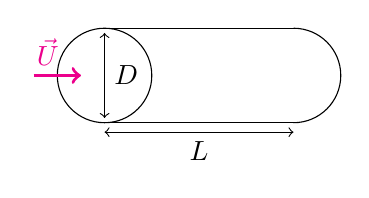
\begin{tikzpicture}[scale=0.6]
        \draw (0,0) circle(1);
        \draw (0,1) -- (4,1);
        \draw (0,-1) -- (4,-1);
        \draw (4,1) arc(90:-90:1); %arc(angle de départ:angle d'arrivée:rayon)
        %L
        \draw [<->] (0,-1.2) -- (4,-1.2);
        \draw (2,-1.2) node[below] {$L$};
        %D
        \draw [<->] (0,0.9) -- (0,-0.9);
        \draw (0,0) node[right] {$D$};
        %U
        \draw [magenta,->,very thick] (-1.5,0) -- (-0.5,0);
        \draw [magenta] (-1.2,0) node[above] {$\vec U$};
    \end{tikzpicture}
\end{center}
%
Pour un écoulement incompressible d'un fluide newtonien en régime \textbf{laminaire} dans une conduite de diamètre $D$ et de longueur $\Delta L$, on peut montrer analytiquement que :
%
\begin{equation}
\Delta p_f = \frac{2\rho U^2}{D} f \Delta L \quad\text{avec } f = \frac{16}{Re}
\end{equation}

$f$ est le coefficient de friction de Fanning. L'expression de $\Delta p_f$ en fonction de $f$ reste valable en dehors des hypothèses précédentes, elle est donc valable pour des fluides non newtoniens et quelque soit le régime d'écoulement. Ce qui changera pour ces cas sera la définition du coefficient de friction $f$. On notera aussi que pour des conduites en anneaux, la définition de $\Delta p_f$ peut être reprise avec $D = D_h$ diamètre hydraulique.

Il existe une autre description du coefficient de friction : celle de Darcy (1856) (ou Moody dans certaines publications), la relation entre coefficient de Darcy et Fanning est très simple :
%
\begin{equation}
f_{\text{Darcy}} = 4\cdot f_{\text{Fanning}}
\end{equation}

Pour un régime \textbf{turbulent}, le coefficient de friction de Fanning vérifie l'équation suivante dite de Colebrook (1939) :
%
\begin{equation}
\frac{1}{\sqrt{f}} = -4\cdot\log\left(0.269~\frac{\epsilon}{d} + \frac{1.255}{Re\sqrt{f}}\right)
\end{equation}
%
Cette formulation est implicite ($f$ se situe des 2 côtés de l'équation) et fait intervenir la rugosité de la paroi de la conduite $\epsilon$ (en $m$). Cette équation se résout avec une méthode itérative (type Newton-Raphson). De nombreuses écritures explicites (donc plus simples mais approximatives) du coefficient de friction ont été formulées. On peut les trouver sur \href{https://en.wikipedia.org/wiki/Darcy_friction_factor_formulae}{Wikipédia}, la plus connue est celle de Blasius (1913) :
%
\begin{equation}
f = \frac{0.0791}{Re^{0.25}}
\end{equation}
